\section{Prediction for unassociated source in the 4FGL catalog}
\lb{sec:4FGLprediction}

After having perused the 3FGL data we moved on to the 4FGL associated data. The 4FGL catalog has higher number of features, especially due to the difference in modeling when compared with the 3FGL. We selected 31 of these features and looked for the corelation between them. If Any feature was corelated or anti-corelated with a pearson index of $\pm$0.75 or higher with another, then only one of them was kept. This resulted in 17 features making it through in the end, which includes 10 of the original features we had used in the 3FGL catalog. The full corelation matrix with indices can be seen below.\\

\begin{figure*}[h]
\centering
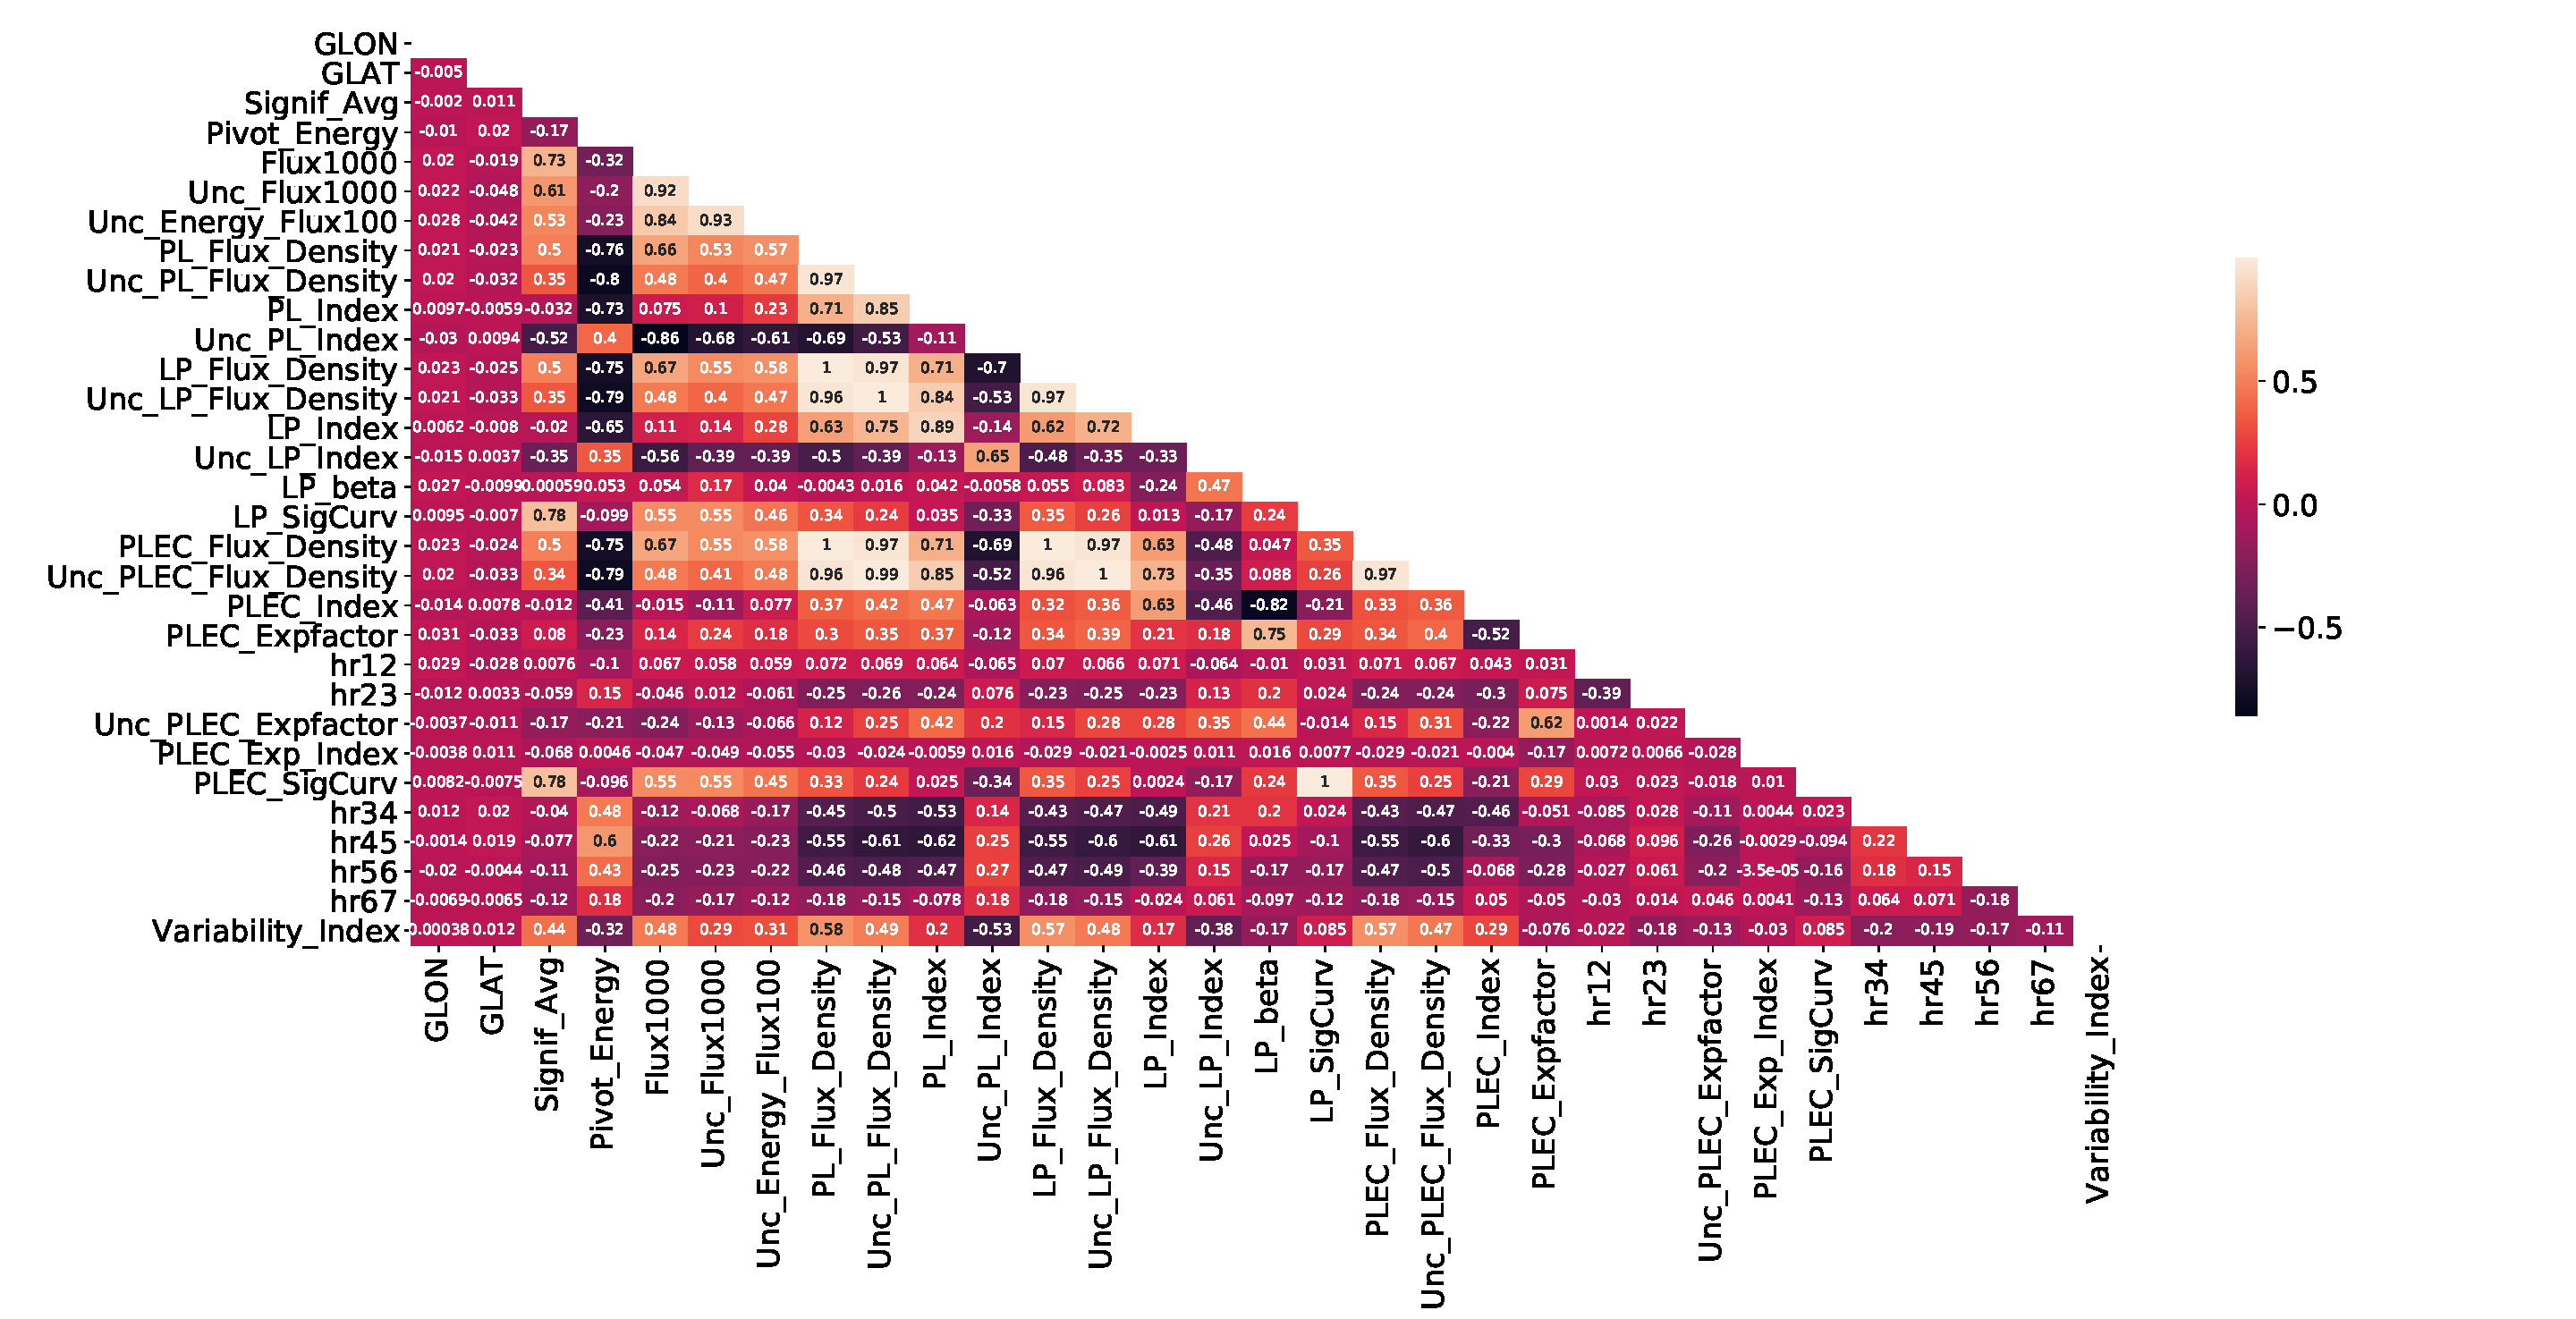
\includegraphics[width=\textwidth]{plots/correlation_4fgl_assoc.pdf}
%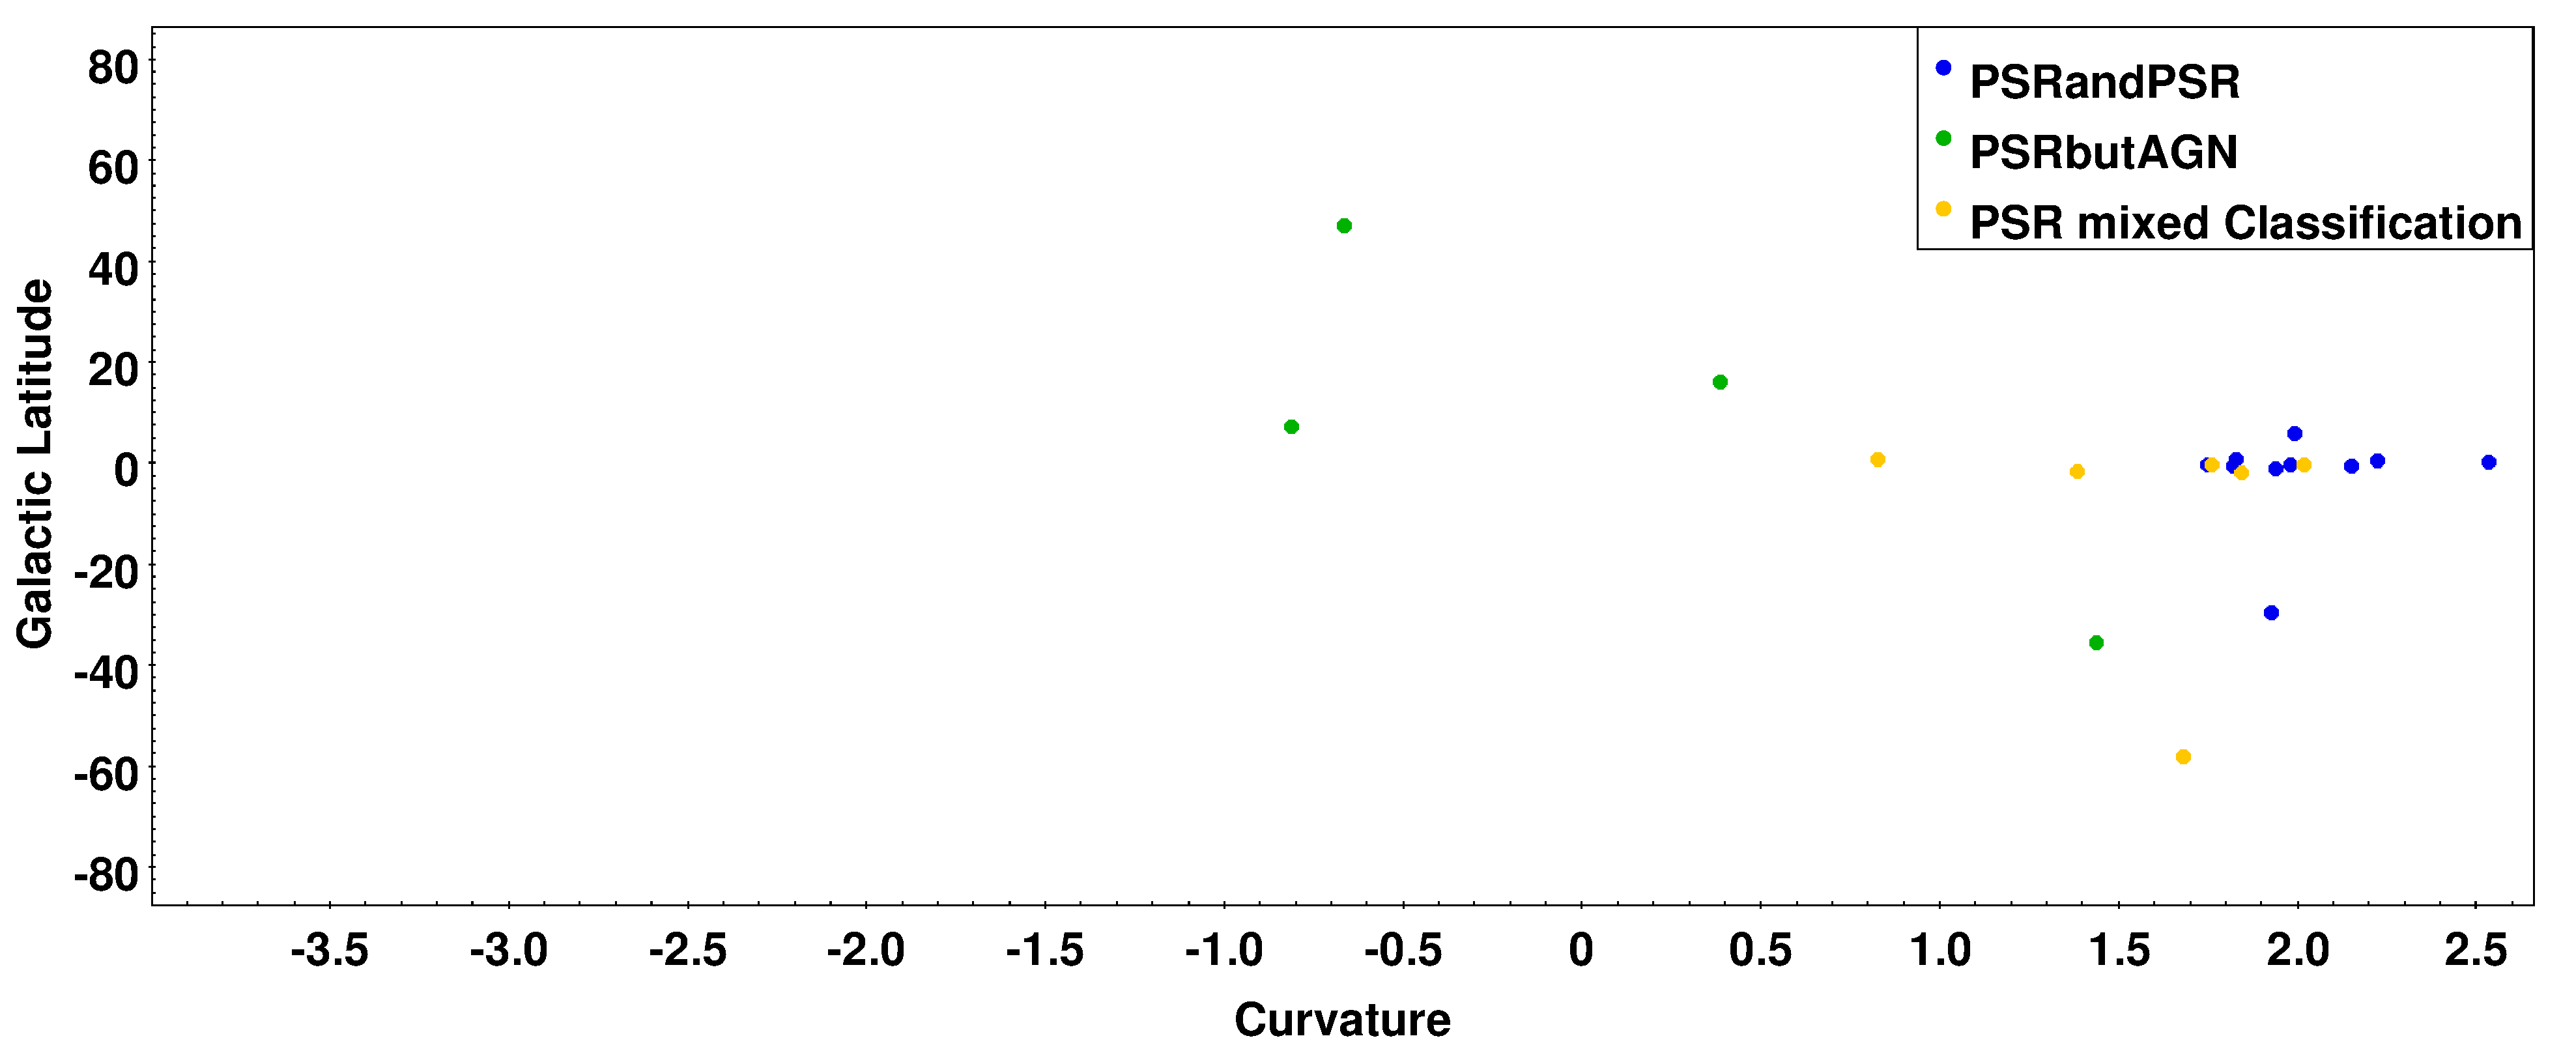
\includegraphics[width=\twopicsp\textwidth]{plots/PSR3.pdf}
\caption{Corelation matrix for 4FGL associated data }
%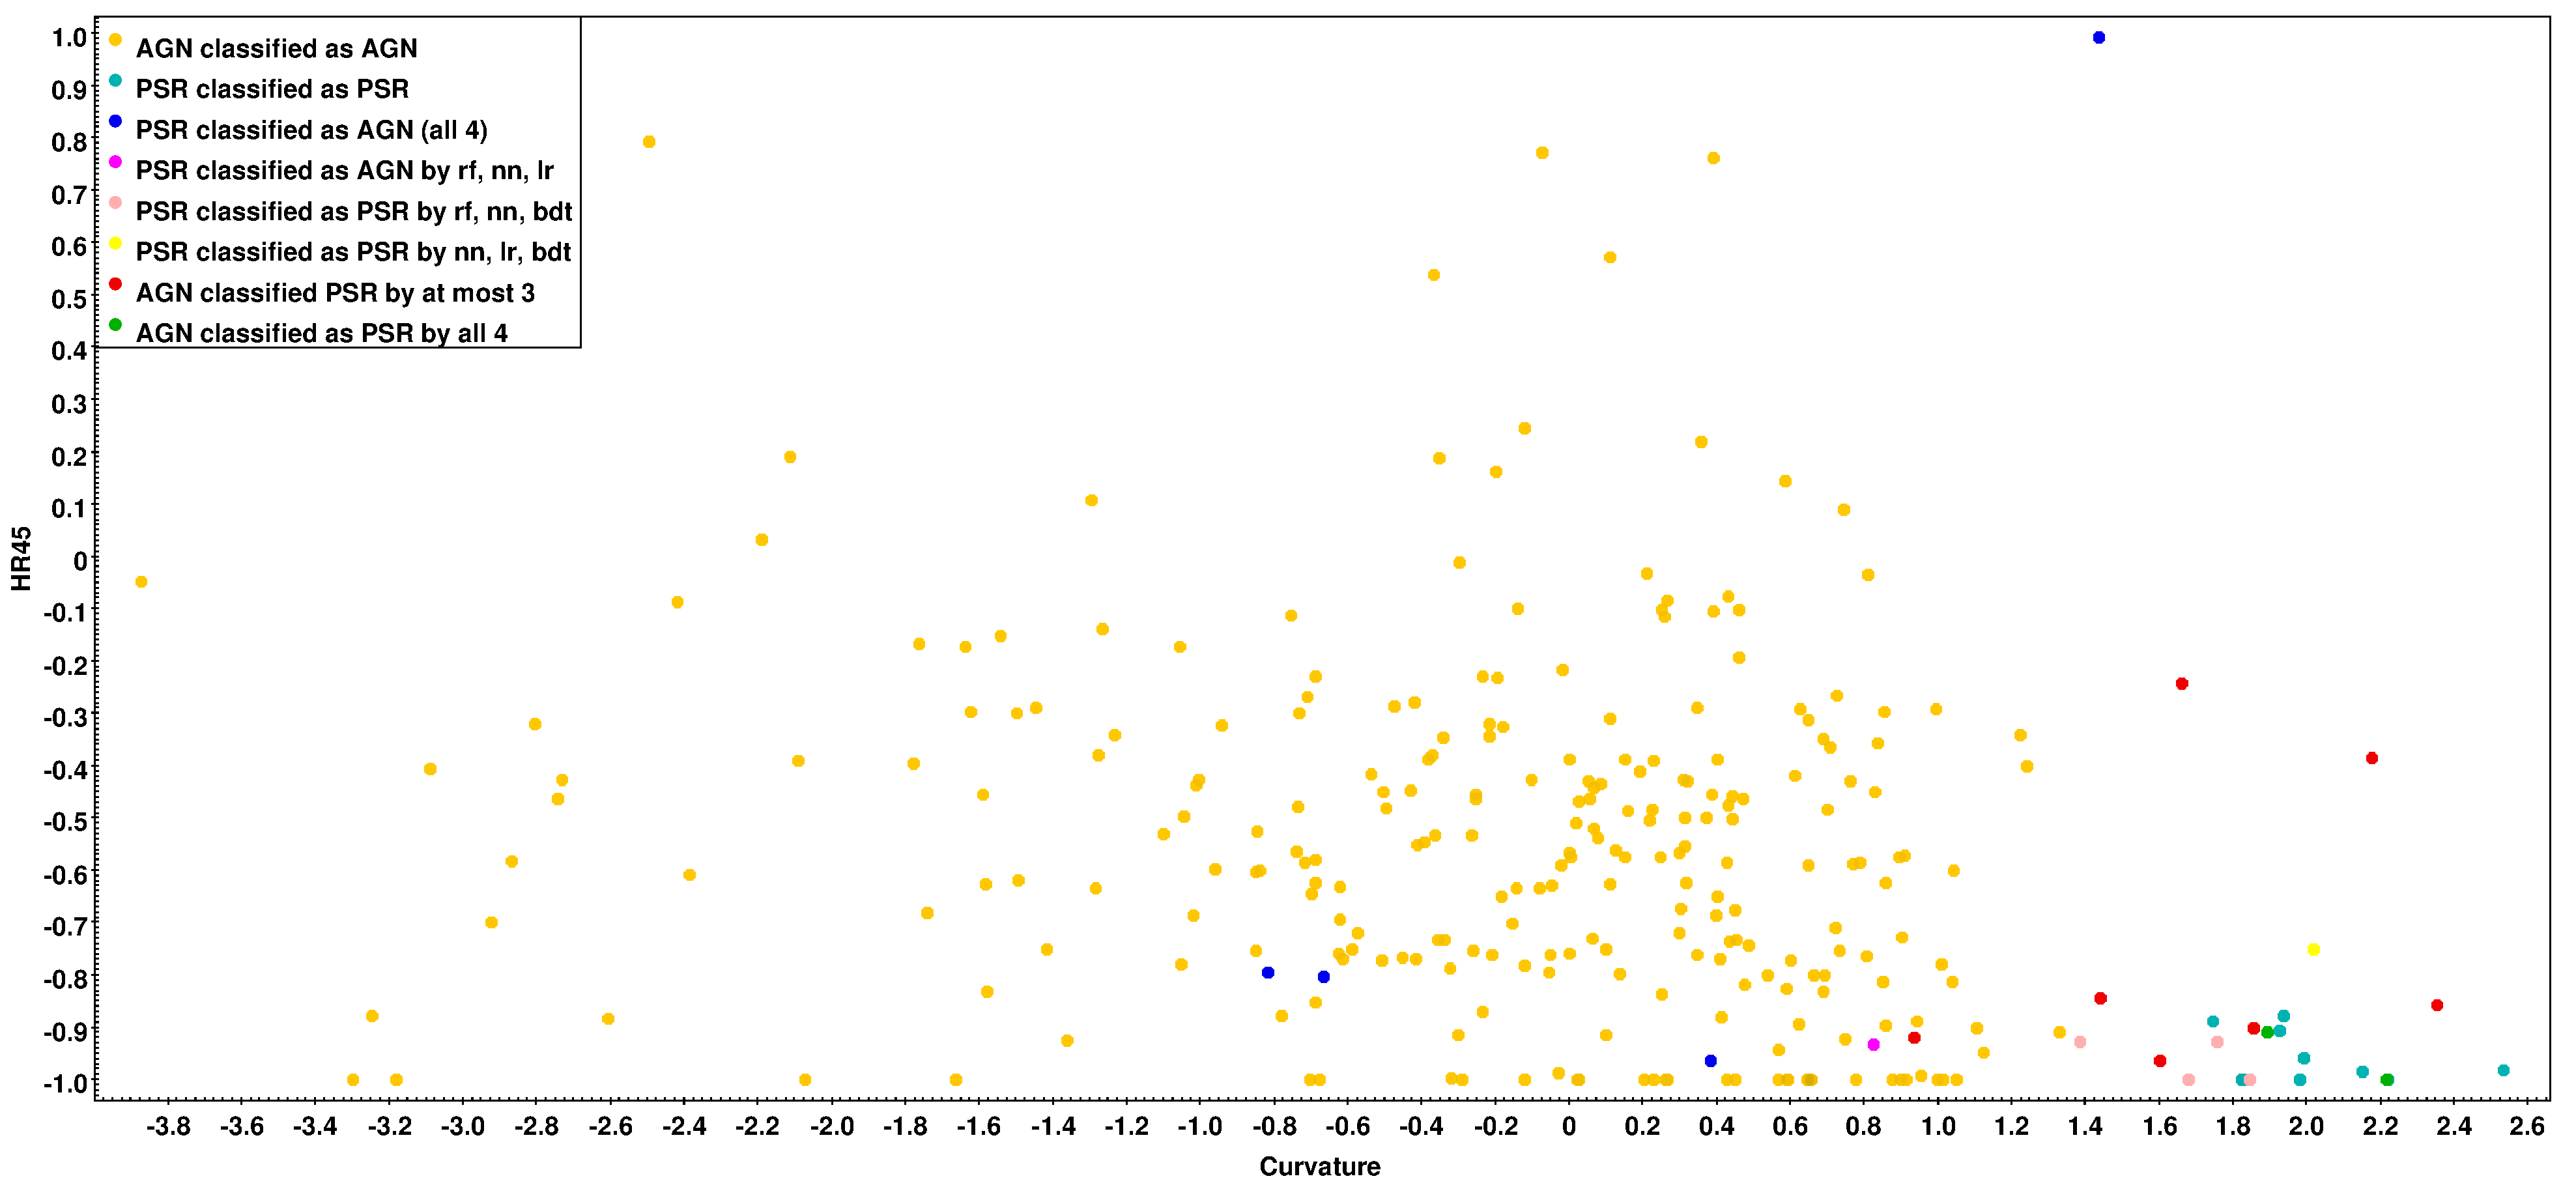
\includegraphics[width=\twopicsp\textwidth]{plots/final_catalog.pdf}
\label{fig:Maps_data}
\end{figure*}

\pgfplotstableread[col sep=comma]{data/4fglassocfeatures.csv}\tableaf
\begin{table}
\resizebox{0.45\textwidth}{!}{
\pgfplotstabletypeset[
columns={Name,Mean,SD,Minimum,Maximum},
column type=c,
string type,
every head row/.style={before row=\toprule,after row=\midrule,},
every last row/.append style={after row={\hline} },
every first column/.style={column type/.add={|}{}},
every last column/.style={column type/.add={}{|}},
columns/Name/.style={column name=Feature Name,string replace*={_}{\textunderscore}},
columns/Mean/.style={column name=Mean,column type=c,numeric type,fixed,precision=2},
columns/SD/.style={column name=Standard Deviation,numeric type,fixed,precision=2},
columns/Minimum/.style={column name=Minimum,numeric type,fixed,precision=2},
columns/Maximum/.style={column name=Maximum,numeric type,fixed,precision=2},
skip rows between index={17}{28}
]{\tableaf}
}
\vspace{0.2cm}
\caption{Statistics for finalized features from 4FGL}
\end{table}

In this section, we chose not to do another preliminary analysis of the algorithms. Therefore we used the same chosen algorithms as before. However, due to the number of features being higher, we hypothesized that the Neural Network should under-perform as compared to before. 
\begin{table}[!h]

\resizebox{0.45\textwidth}{!}{
    \tiny
 %  \centering
    \renewcommand{\tabcolsep}{0.3mm}
\renewcommand{\arraystretch}{1.5}

    \begin{tabular}{|c|c|c|}
    \hline
    Algorithm&Parameters & Training Accuracy \\
    \hline
    RF& 50 trees, max depth 6  &98.27\\
    \hline
    NN & 300, 10 Neurons, Adam & 95.36\\
    \hline %\midrule   -> aakash do you mean this?
    BDT & 100 trees, max depth 2    &   98.23\\
%    \hline %\midrule   -> aakash do you mean this?
%    BDT & 200 trees, max depth 2    &   95.8  \\
    \hline
    LR & LBFGS solver, 200 iterations & 98.08\\
    \hline
     
    \end{tabular}}
    \vspace{0.2cm}
    \caption{Accuracy of the 4 selected algorithms on 4FG associated data.}
    \label{tab:selected_algs2}
\end{table}

As can be seen in the table above, all algorithms except the Neural Network perform better, reaching more than 98\% accuracy. 